\documentclass[12pt, a4paper]{article}
\usepackage[margin=0.5in]{geometry}
\usepackage{multicol}
\usepackage{authblk}
\usepackage[hidelinks]{hyperref}
\usepackage{graphicx}
\graphicspath{ {assets/img/} }
\usepackage{float}
\usepackage{polyglossia}
\setdefaultlanguage{english}
\setotherlanguage{sanskrit}
\usepackage{fontspec}
\setmainfont{Times New Roman}
\newfontfamily{\devanagarifont}[Script=Devanagari]{Lohit Devanagari}
\renewenvironment{abstract}
{\small
	\begin{center}
		\bfseries \abstractname\vspace{-.5em}\vspace{0pt}
	\end{center}
	\list{}{
		\setlength{\leftmargin}{0mm}
		\setlength{\rightmargin}{\leftmargin}
	}
	\item\relax}
{\endlist}
\title{Emotionally Intelligent Machines \& Sentiment Synthesis based on Ancient Vedic Astrology}
\author[1]{Mohit Singh}
\author[2]{Dr. Priyank Singhal}
\author[3]{Mr. Vikas Kuchhal}
\affil[1,2,3]{College of Computing Sciences \& Information Technology\\Teerthanker Mahaveer University\\Moradabad, Uttar Pradesh\\India}
\affil[1]{\href{mailto:mohit.tca2212005@tmu.ac.in}{mohit.tca2212005@tmu.ac.in}}
\affil[1,2,3]{DOI:}
\begin{document}
	\maketitle
	\hrule
	\begin{abstract}
		\textbf{After brain researchers have recognized that emotions are crucial for human and animal intelligence, Artificial Intelligence researchers have also started to acknowledge the importance of emotions in the design of intelligent machines. In this seminar, we will discuss about the Emotionally Intelligent Machines(EIM's) which is the new field of research in Artificial Intelligence but it has a great potential to do immense good, however the technology can be misused but it is up to the consumers of this technology who will decide whether it will be used for good or for evil. Also, Astrology has always been a controversial topic and is completely depends upto the personal faiths and beliefs of an individual. Apart from that, this paper describes that how Emotionally Intelligent Machines(EIM's) \& Sentiment Synthesis Systems can be developed by using the concept of Ancient Vedic Astrology.}
	\end{abstract}
	\textbf{Keywords: }
	Artificial Intelligence(AI), Emotional Intelligence(EI), Emotional Artificial Intelligence(EAI), Intution, Consciousness, Unconsciousness, Subconscious, Belief System, Feed Forward Network(FFN), Recurrent Neural Network(RNN), Convergence, Divergence,%Neural Networks, Sentimental Analysis, Vedic Astrology, Synthesis, Emotional Intelligence, Affective Computing, Subconsious, Cognitive Science, Philosophy, Psychology, Modalities, Galvanic Resistance, Bioinformatics, The Gateway Experience, Hemi-Sync, Cognitive Dissonance, Cognitive Harmony, Astral Travel, Hypnosis, Trasedental Meditation, BioFeedback(Creative Visualization), Emotion Dynamics
	\newline
	\hrule
	\begin{multicols}{2}
		\section{Introduction}
		%For half a century, artificial-intelligence researchers have focused on giving machines linguistic and mathematical-logical reasoning abilities, modelled after the classic linguistic and mathematical-logical intelligences. This paper describes new research that is giving machines skills of emotional intelligence. Machines have long been able to appear as if they have emotional feelings, but they are now being programmed to also learn when and how to display emotion in ways that enable them to appear empathetic or otherwise emotionally intelligent. They are now being given the ability to sense and recognize expressions of human emotion such as interest, distress, and pleasure, with the recognition that such communication is vital for helping them choose more helpful and less-aggravating behaviour.

%Emotionally Intelligent Machines are the systems that can recognize, interpret, process, and simulate human emotions based on the concept of ancient vedic astrology. They are the machines which can adapt different situations and knows how to handle these situations more intelligently and smartly. In modern technical world, the need of EIM's are can be seen due to their numerous applications which are expanding rapidly. Some of the common applications of EIM's are:
		\section{Research Model \& Hypothesis}
		The chapter mainly describes the discussion on relationship between the birth chart 
the mathematics of dynamical systems, ancient vedic astrology \& the psychology of human behaviour which is completely based on the supporting evidences found during the study of Artificial Emotional Intelligence(AEI). Sentiments can be synthesized in machines and algorithms by means of artificial intution based on the concept of ancient vedic astrology which will lead to the development of more smart and intelligent systems. These type of systems can be very helpful in many areas such as in Healthcare, Education, Business Intelligence, Social Media, Automobile, etc.
		\section{Related Work \& Review of Literature}
		\begin{itemize}
	\item
	Need, Importance and benifits of Emotionally Intelligent Machines, What is Emotional Intelligence, Some applicaitons of EI, Limitations of Artificial Intelligence, \cite{ISSN-2456-2165}
	\item 
	
\end{itemize}
		\section{Methodology}
		\begin{figure}[H]
	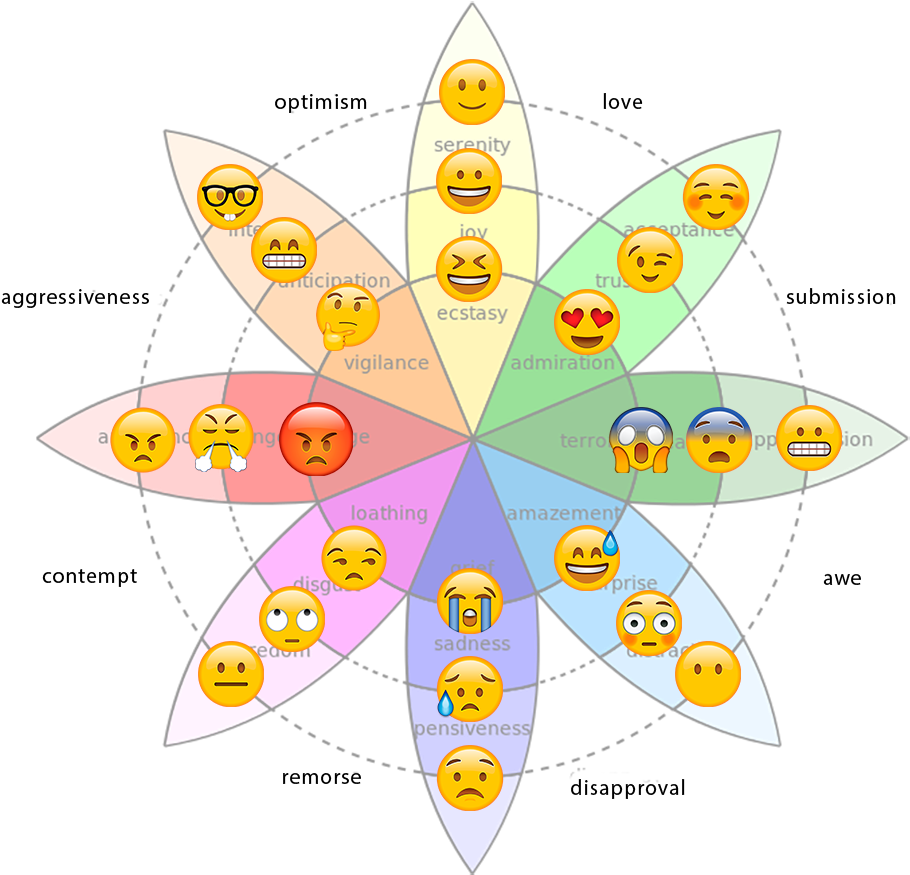
\includegraphics[width=\columnwidth, keepaspectratio]{PWOEEmoji}
	\caption{Plutchik's Wheel of Emotions Emojis}
	\label{Fig:fig4}
\end{figure}
Figure \ref{Fig:fig4} shows PWOE with Emojis.
		\section{Implementation \& Planned Experiments}
		\input{assets/Implementation}
		\section{Conclusion \& Outlook}
		The human mind is a very complex dynamical system that evolves over time in responses to the various inputs from the environment. The more we attempt to understand it deeply, the more we find ourselves entangled in questions. However, this pursuit provides us with new knowledge that leads to innovation and presents numerous challenges. The study of the human mind has been instrumental in the birth of artificial intelligence (AI), but there still exists a significant difference between AI and the human mind. To bridge this gap, psychology and Vedic astrology can play a crucial role, and by leveraging these theories, intuition-based AI systems could be developed in the future.
	\end{multicols}
	\hrule
	\centering
	\section*{Summary}
	The human mind is a very complex dynamical system that evolves over time in responses to the various inputs from the environment. To understand this in simple words, let's imagine what will happen if human mind does not have any type of memory with it or it will act as a static system. What will be our experience in this case? How does it feel like? If it will be the case, then everything will be instantaneous for us. There is no happieness, no sadness no fear \& no anger. There will be no emotions. There will be no experience of feeling anything due to the absence of memory. This will happen because our mind collects all the past experiences of our life as data in the memory and whenever will be a situation to deal, it extracts the information of the past experiences stored inside the memory, compares this information with the present input, and decides how to handle with and react in this situation. This task handling experience is stored again in the memory for the future processing.
	\section*{Acknowledgements}
	\textit{``I would like to express my sincere gratitude to all those who have contributed to the completion of this research paper. Firstly, I am very grateful to my supervisors Dr. Priyank Singhal \& Mr. Vikas Kuchhal, my mentor Dr. Anu Sharma and jyotishachrya Mr. DK Lahori for providing me the guidance and support throughout the research. Their feedback, encouragement, and insightful comments have been invaluable in shaping this paper."}

\textit{``I am very grateful to Dr. RK Dwivedi the director of College of Computing Sciences \& Information Technology for providing me the opportunity to conduct this research as part of my academic program. This research has not only been a valuable learning experience but has also contributed to the knowledge base of the field."}

\textit{``I would also like to thank my colleagues and friends who provided me with valuable feedback and suggestions on the initial drafts of this paper. Their inputs have significantly improved the quality of this research."}

\textit{``Furthermore, I would like to express my gratitude to Teerthanker Mahaveer University for providing me the necessary resources and infrastructure to conduct this research. The library staff and resources have all played an integral role in the successful completion of this study."}

\textit{``The research skills and knowledge I have gained during my time at the college have been instrumental in shaping my approach to this research. I would also like to acknowledge the faculty members who have taught and mentored me during my academic journey, their insights and teachings have been invaluable in shaping my research skills and approach."}

\textit{``I am grateful to have had the opportunity to study at such an esteemed institution and to have been surrounded by individuals who have pushed me to achieve my best. Thank you, Teerthanker Mahaveer University, for contributing to my academic and personal growth."}

\textit{``Finally, I would like to thank my family for their unwavering support and encouragement throughout the research. Their love and understanding have been a source of strength and inspiration to me."}

\textit{``Once again, thank you to everyone who has contributed to this research."}
	\newline
	\hrule
	\bibliography{assets/Citations}
	\bibliographystyle{acm}
	\section*{Annotated Bibliography}
	\appendix
	\section*{Appendix}
	\listoftables
\listoffigures
\section{\\Title of Appendix A}
% the \\ insures the section title is centered below the phrase: AppendixA

Text of Appendix A is Here

\section{\\Title of Appendix B}
% the \\ insures the section title is centered below the phrase: Appendix B

Text of Appendix B is Here
\end{document}